\chapter{Mitigation Framework}
\label{chap:mitigation}

In the event of a comet remnant impact, the impacting material is likely to often pass perihelion (and thus approach impact with the Earth) on the order of a few years after discovery. In the most extreme examples, highly eccentric LPC nuclei may only become visible once within the orbit of Jupiter - leaving only a few months' time to react. 

Therefore, strategies that mitigate against Earth-bound cometary material are of a different nature to the more popular proposed planetary defence efforts that focus primarily on asteroids. Such strategies focus on mitigating against high energy objects with a short warning time. Recent discussions of direct comet mitigation in literature range from the use of large phased-array lasers illuminating LPC nuclei from afar \citep{2016PASP..128d5001Z}, to a nuclear explosive device affixed to an interceptor craft that waits in stand-by in an orbit around Earth \citep{7500925, HUSSEIN2016488}. %A nuclear detonation is one of the few plausible mitigation strategies that could sufficiently deflect a comet away from Earth, and even then may only be feasible if sent to meet the comet almost immediately upon discovery. 

However in this paper we advocate a more detection-based approach, developing a random forest classification model to detect hazardous evolving cometary material scattered in the Solar System from our current catalogues of small bodies detected from Earth. Such a framework may permit a greater understanding of the nature of hazardous cometary material presently being scattered through the Solar System, and therefore inform us on how best to develop a response.

We develop a mitigation framework that acts purely on the dynamical qualities of a comet's orbit, and neglects features such as a comet's size and other physical attributes. In developing a detection method to look for evidence of dangerous cometary material, regardless of size, composition etc - we hope to look for cometary remnants that could themselves be an direct threat to Earth, or that could be genetically associated with an as of yet unobserved threatening parent comet nuclei or host of fragmented material.

\begin{figure}[t!]
    \centering
    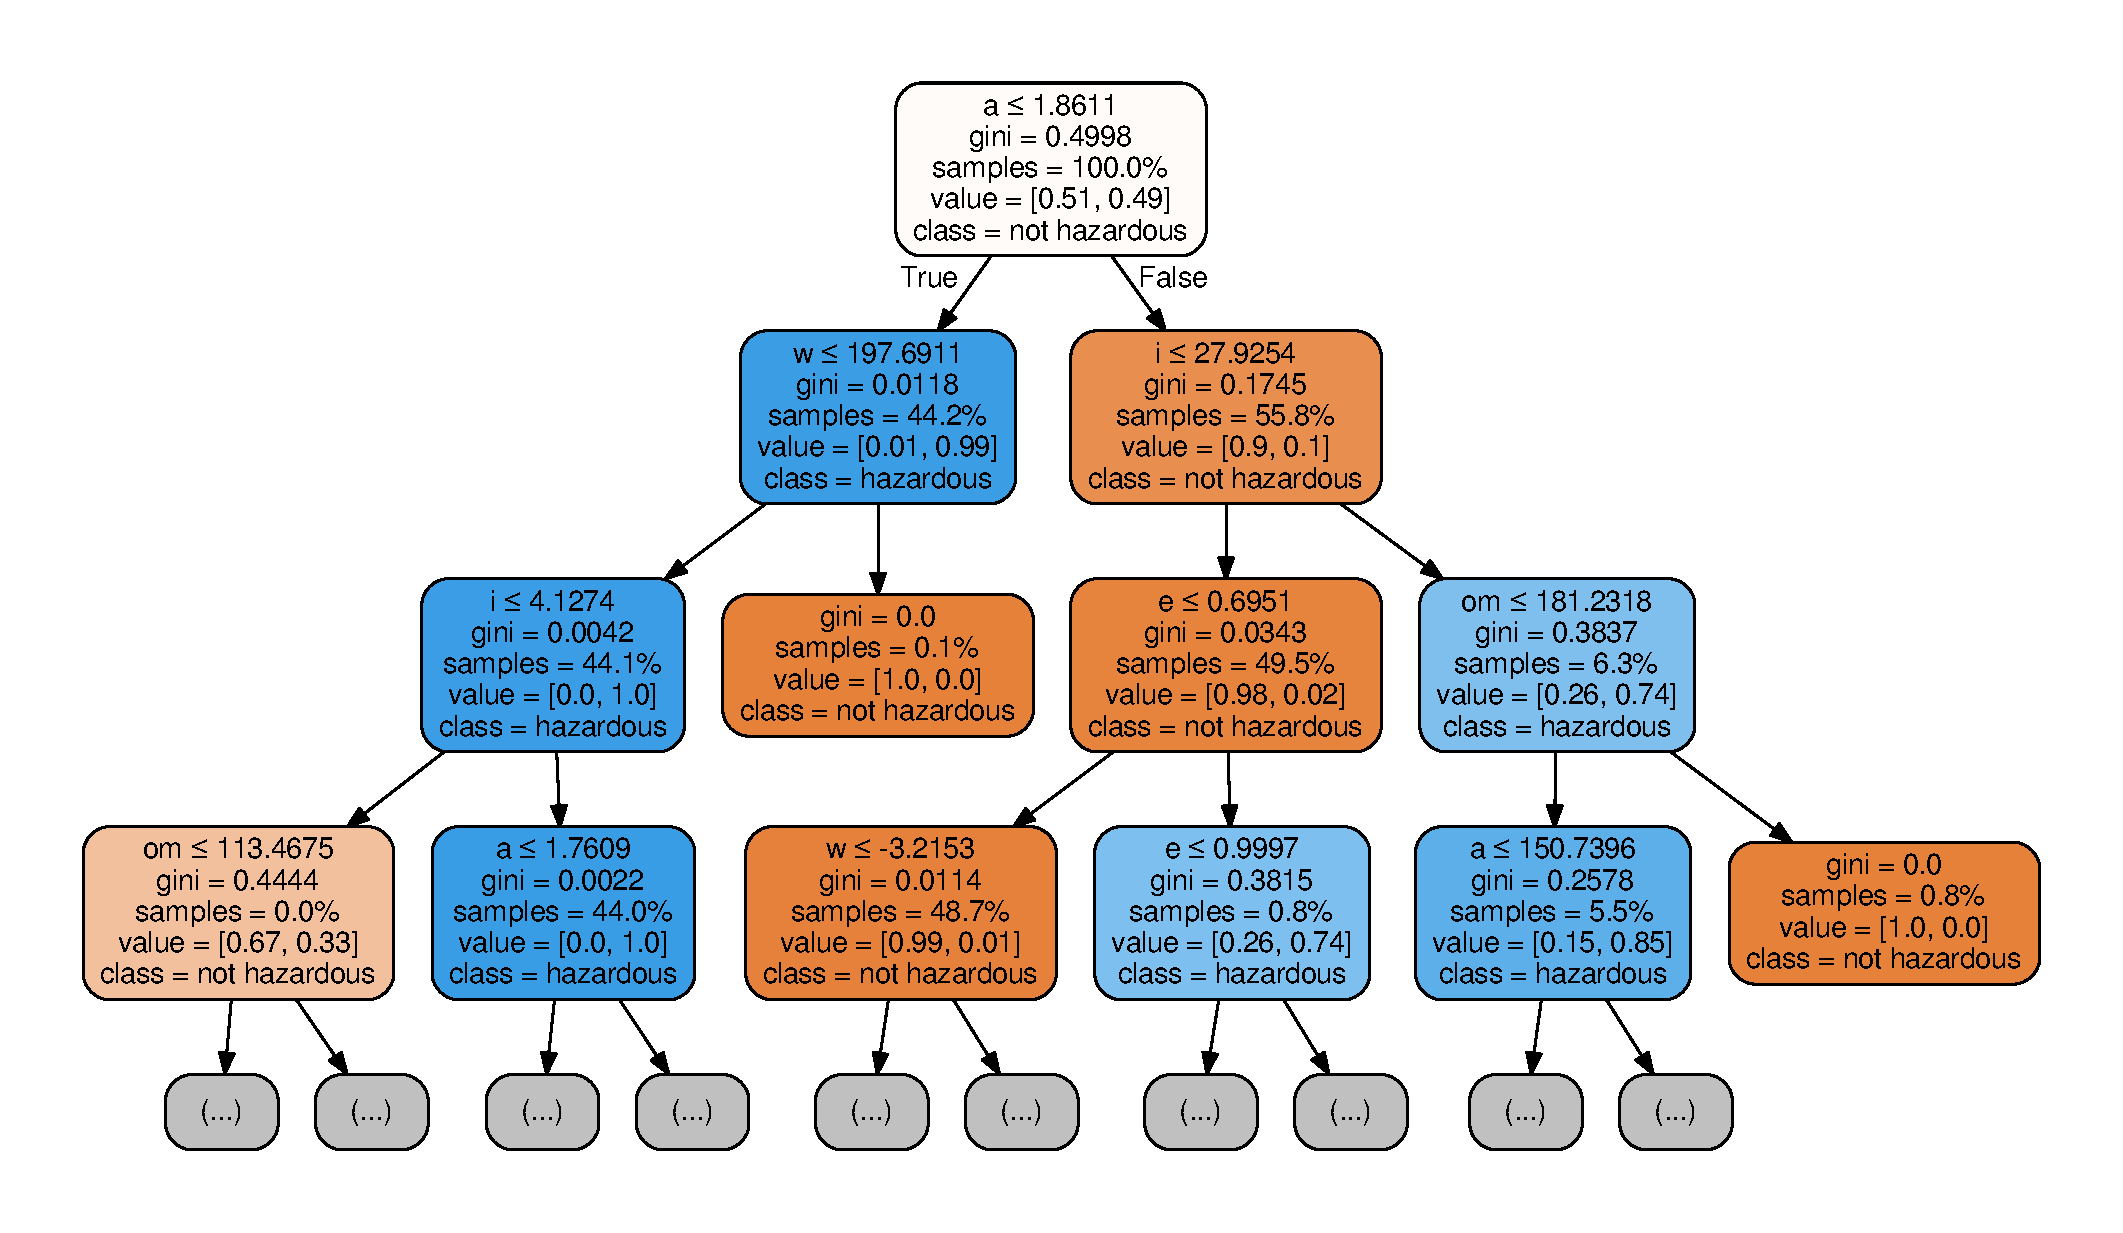
\includegraphics[trim={0 0 0 1cm}, clip, width=0.95\textwidth]{tree1.pdf}
    \caption[Example decision tree]{Example decision tree used in the random forest, expanded for the first few layers. Samples represent the percentage of training datapoints associated with a particular node. Values show the fraction of records for each class that have reached that node particular node. The node fill colour denotes the majority class for classification. `om' and 'w' denote longitude of ascending node $\Omega$ and argument of perihelion $\omega$ respectively.}
    \label{fig:tree}
\end{figure}

\section{Random Forest Model}

While N-body integrations help us understand the various dynamical pathways that a comet may take, they are inherently computationally intensive and time consuming processes; this makes them unsatisfactory for examining the long-term evolution of individual specific objects and how they may pose a risk to our planet.

We instead select a large sample of orbital features from our N-body simulation, and use this to train a predictive model in order classify objects with similar orbital characteristics as hazardous. Hazardous orbits from the simulation are used in a learning algorithm alongside non-hazardous orbits with more asteroidal dynamical characteristics - sourced from the JPL small body database.

We selected a large number of datapoints from our simulation data at various points in time. In particular we selected simulated comets that i) entered the Earth's loss cone only once ii) spent most of their dynamical lifetimes beyond the orbit of Jupiter iii) were initially bound to the Solar System at the beginning of the simulation. This selection was chosen in order to prioritise cometary material that could represent the dominant impact hazard, ie. those that rapidly and chaotically evolve through the Solar System, and arrive in the NEO environment with short warning times. From this selection of datapoints we used an 8:2 split for training and validation purposes respectively.

The random forest classification model is made up of an ensemble of many classification decision trees, which themselves individually separate the feature space of a training data set into smaller and smaller partitions. Individual decision trees have a habit of learning a dataset to such a degree that corresponds too closely to that particular dataset. This makes individual trees `weak learners' - meaning that they are prone to `overfitting' and can fail to fit additional data or predict future observations once fully trained. In an attempt to limit a decision tree's ability to `overfit' to the data it's been trained on, we aggregate a number of decision trees into one final structure known as a random forest. Random forests consist of the averaged ensemble of decision trees that have all individually been trained on random subsets of the training data.

We implement our random forest using the \textsc{CART} decision tree algorithm \citep{breiman2017classification} from the \texttt{Python} library \texttt{scikit-learn} \citep{cournapeau2015sci}. During the training process, at the point of a particular feature partition, the algorithm maximises the efficiency of a tree such that the Gini impurity $I_G$ of the two resulting feature partitions is minimised. The Gini impurity can be calculated by summing the probability $p_f$ of an item with label $f$  being chosen multiplied by the probability of a mistake in categorising that item.  It is given by,

\vspace{-1ex}
\begin{equation}
   I_G =  \sum_{k = 0}^k p_f(1-p_f)~,
\end{equation}

where $k$ is the number of classes. For our model we use $k=2$, where the two classes denote hazardous cometary material and non-hazardous material. 

We trained our random forest algorithm using five orbital elements as features. These were $(a,e,i,\Omega,\omega)$ - semi-major axis, eccentricity, inclination, longitude of ascending node, and argument of perihelion respectively. These features completely describe the shape and orientation of a comet's orbit relative to the Sun, neglecting the comet's particular position in time. These features therefore encode all the necessary information (for example velocity, value of $T_J$) that permit a classification on whether the object is hazardous or not.

We constructed a random forest of 100 individual trees, trained with a maximum depth of 6 levels. With a trained random forest, orbital elements were then propagated through the structure and a predicted classification was then output.

\section{Results}

Our model performed well against our validation data, with 77\% of results predicting a hazardous orbit being correct, with 85\% of the hazardous comets classified successfully.

Unlike other predictive models which have more of a black box nature, each trained decision tree in our random forest could be individually studied and interpreted. One decision tree used in the learning process is shown in Fig.~\ref{fig:tree}, which illustrates one example of how a random subset of the training data was partitioned at each node. A feature is chosen at each decision node that minimises $I_G$, such that it best segregates the the two classes. The tree continues partitioning until $I_G$, or the maximum number of permitted levels is reached.

By examining the total reduction of $I_G$ due to a particular feature across all our decision trees, we were able to calculate the relative importance of each feature used for classification. We found that $e$ was the most important determining feature of an object's orbit as to whether it is hazardous or not, at a relative importance of 0.42. The next most important determining features were $a$ and $i$, providing support to the use of $T_J$ as a dynamical classifier.

Having now trained the random forest, the classifier was then applied to all known small bodies as catalogued by the JPL small body database, around 192 ($\sim0.1\%$) of the objects were classed as having similar orbital evolutionary characteristics as the dangerous comets in our simulation. This group of objects were made up 70\% LPCs, 19\% SPCs, 11\% eccentric asteroids and minor planets - all at various stages in their dynamical evolution. Notable classifications included; the NEO 4341 Poseidon - associated with the Taurid Complex of meteor showers \citep{2001A&A...373..329B}, 944 Hidalgo - one of the first Centaurs to be discovered, and 109P/Swift-Tuttle - described by \cite{verschuur1997impact} as the `the single most dangerous object known to humanity'.

The random forest provided a human-interpretable, generalisable, and fast classification tool that proved effective at identifying real objects orbitally evolving in a similar fashion to the exceptionally hazardous and dynamically realistic impactors that were selected from our simulation. One limitation was that the non-hazardous class was trained on objects not derived from our simulation. Due to the inherent observation biases present in real observation data, it is encouraged that future predictive models adopt a one-class classification learning approach. This would allow one to discriminate a class of dynamical objects from an outlier class, with no prior knowledge about the outlier class.

%Notable classifications include objects on eccentric orbits that are already classified as NEOs and are therefore relevant to the human epoch. These included the NEOs 2003 EH1, 2004 UL, and 2004 TG$_{10}$. The notable 109P/Swift–Tuttle comet was classified as hazardous.

%https://www.repository.cam.ac.uk/bitstream/handle/1810/246615/MNRAS-2015-Shannon-2059-64.pdf?sequence=1 read S5